% This is "sig-alternate.tex" V2.0 May 2012
% This file should be compiled with V2.5 of "sig-alternate.cls" May 2012
%
% This example file demonstrates the use of the 'sig-alternate.cls'
% V2.5 LaTeX2e document class file. It is for those submitting
% articles to ACM Conference Proceedings WHO DO NOT WISH TO
% STRICTLY ADHERE TO THE SIGS (PUBS-BOARD-ENDORSED) STYLE.
% The 'sig-alternate.cls' file will produce a similar-looking,
% albeit, 'tighter' paper resulting in, invariably, fewer pages.
%
% ----------------------------------------------------------------------------------------------------------------
% This .tex file (and associated .cls V2.5) produces:
%       1) The Permission Statement
%       2) The Conference (location) Info information
%       3) The Copyright Line with ACM data
%       4) NO page numbers
%
% as against the acm_proc_article-sp.cls file which
% DOES NOT produce 1) thru' 3) above.
%
% Using 'sig-alternate.cls' you have control, however, from within
% the source .tex file, over both the CopyrightYear
% (defaulted to 200X) and the ACM Copyright Data
% (defaulted to X-XXXXX-XX-X/XX/XX).
% e.g.
% \CopyrightYear{2007} will cause 2007 to appear in the copyright line.
% \crdata{0-12345-67-8/90/12} will cause 0-12345-67-8/90/12 to appear in the copyright line.
%
% ---------------------------------------------------------------------------------------------------------------
% This .tex source is an example which *does* use
% the .bib file (from which the .bbl file % is produced).
% REMEMBER HOWEVER: After having produced the .bbl file,
% and prior to final submission, you *NEED* to 'insert'
% your .bbl file into your source .tex file so as to provide
% ONE 'self-contained' source file.
%
% ================= IF YOU HAVE QUESTIONS =======================
% Questions regarding the SIGS styles, SIGS policies and
% procedures, Conferences etc. should be sent to
% Adrienne Griscti (griscti@acm.org)
%
% Technical questions _only_ to
% Gerald Murray (murray@hq.acm.org)
% ===============================================================
%
% For tracking purposes - this is V2.0 - May 2012
\documentclass{sig-alternate}
\setlength{\pdfpagewidth}{8.5in}

\setlength{\pdfpageheight}{11in}

\usepackage{textcomp}
\usepackage{hyperref}
\hypersetup{pdfpagemode=UseNone}
\usepackage{subfig}
\usepackage{booktabs}
\usepackage{multirow}
%\usepackage{natbib}
\usepackage{color,soul}
\usepackage{enumitem}
\usepackage{balance}

%\usepackage{amsmath,scalerel}

%\DeclareMathOperator*{\Bigcdot}{\scalerel*{\cdot}{\bigodot}}

\newtheorem{cond}{Condition}
\newtheorem{defn}{Definition}

\usepackage{etoolbox}

\usepackage{microtype}

\usepackage{fixltx2e}


%command to comment out stuff
\newcommand{\comment}[1]{}

%space saving!!!
%\comment{
\addtolength{\textfloatsep}{-10pt}
\addtolength{\floatsep}{-7pt}
\addtolength{\abovecaptionskip }{-5pt}
\addtolength{\dbltextfloatsep}{-7pt}
\addtolength{\dblfloatsep}{-5pt}

%Change caption size to small
\renewcommand{\captionfont}{\small}
\renewcommand{\captionlabelfont}{\small}

%reduce space between bib entries -- requires natbib
%\setlength{\bibsep}{0.04cm}

%use 0.95 or higher
\linespread{0.93}

\setlist[itemize]{leftmargin=*}
\setlist[enumerate]{leftmargin=*}


%}

\begin{document}
\makeatletter
\patchcmd{\@afterheading}%
    {\clubpenalty \@M}{\clubpenalties 3 \@M \@M 0}{}{}
\patchcmd{\@afterheading}%
    {\clubpenalty \@clubpenalty}{\clubpenalties 2 \@clubpenalty 0}{}{}
\makeatother
\sloppy
%
% --- Author Metadata here ---
\conferenceinfo{FPGA}{'15, February 22--24 2015, Monterey, CA, USA}
\CopyrightYear{2015} % Allows default copyright year (20XX) to be over-ridden - IF NEED BE.
\crdata{978-1-4503-3315-3/15/02\\
http://dx.doi.org/10.1145/2684746.2689074}  % Allows default copyright data (0-89791-88-6/97/05) to be over-ridden - IF NEED BE.


% --- End of Author Metadata ---


%--------------------------------------------------------------------------------------------
% Custom commands
%--------------------------------------------------------------------------------------------

%\renewcommand{\footnoterule}{%
%  \kern -3pt
%  \hrule width 0.49\textwidth height 0.5pt
%  \kern 2pt
%} 

\newcommand{\til}{{\fontfamily{ptm}\selectfont\texttildelow}}
\newcommand{\xx}{$\times${ }}

%shortcut command for pdf figures
\newcommand{\fig}[3]{\begin{figure}[t]
\centering
\includegraphics[width=2.5in,#2]{images/#1}
\caption{#3}
\label{#1}
\end{figure}}

%shortcut command for pdf figures
\newcommand{\figg}[4]{\begin{figure}[t]
\centering
\includegraphics[width=#2,#3]{images/#1}
\caption{#4}
\label{#1}
\end{figure}}

%shortcut command for pdf figures
\newcommand{\figc}[3]{\begin{figure}[t]
\centering
\includegraphics[width=1.0\columnwidth,keepaspectratio,#2]{images/#1}
\caption{#3}
\label{#1}
\end{figure}}

%shortcut command for pdf figures
\newcommand{\figch}[3]{\begin{figure}[h]
\centering
\includegraphics[width=1.0\columnwidth,keepaspectratio,#2]{images/#1}
\caption{#3}
\label{#1}
\end{figure}}


%shortcut command for pdf figures
\newcommand{\figvs}[4]{\begin{figure}[!t]
\centering
\includegraphics[width=#1\columnwidth,keepaspectratio,#3]{images/#2}
\caption{#4}
\label{#2}
\end{figure}}

%shortcut command for pdf figures
\newcommand{\figvsh}[4]{\begin{figure}[!h]
\centering
\includegraphics[width=#1\columnwidth,keepaspectratio,#3]{images/#2}
\caption{#4}
\label{#2}
\end{figure}}


%shortcut command for pdf figures
\newcommand{\figfull}[4]{\begin{figure*}[!t]
\centering
\includegraphics[width=#1\columnwidth,keepaspectratio,#3]{images/#2}
\caption{#4}
\label{#2}
\end{figure*}}

%shortcut command for pdf figures with placement hint
\newcommand{\figp}[4]{\begin{figure}[#4]
\centering
\includegraphics[width=2.5in,#2]{images/#1}
\caption{#3}
\label{#1}
\end{figure}}

%adding subsubsubsection
\newcommand{\subsubsubsection}[1]{\vspace{0.2cm}\noindent\textbf{\textit{#1:}}}



%--------------------------------------------------------------------------------------------
% Title
%--------------------------------------------------------------------------------------------

\title{Designing with a NoC-Enhanced FPGA} 
\title{Take the Highway:\\
Design and Simulation for a NoC-Enhanced FPGA} 
\title{Take the Highway:\\
Design and Simulation for Embedded NoCs on FPGAs} 
\title{Take the Highway:\\
Design for Embedded Networks-on-Chip on FPGAs} 
\title{Take the Highway:\\
Design for Embedded NoCs on FPGAs} 
\title{Take the Highway: Design for Embedded NoCs on FPGAs} 

%\subtitle{--blind submission--}

%\comment{

\numberofauthors{1} %  in this sample file, there are a *total*
% of EIGHT authors. SIX appear on the 'first-page' (for formatting
% reasons) and the remaining two appear in the \additionalauthors section.
%
\author{
% 1st. author
\alignauthor
Mohamed S. Abdelfattah, Andrew Bitar, Vaughn Betz\\\vspace{.15cm}
       \affaddr{Department of Electrical and Computer Engineering}\\\vspace{.03cm}
       \affaddr{University of Toronto, Toronto, ON, Canada}\\\vspace{.04cm}
       \email{\{mohamed, bitar, vaughn\}@eecg.utoronto.ca}
}

%}%end of commented block


\maketitle


%
%#############################################################
% ABSTRACT
%-0-0-0-0-0-0-0-0-0-0-0-0-0-0-0-0-0-0-0-0-0-0-0-0-0-0-0-0-0-0-
%
\begin{abstract}
%
%
\comment{
\hl{change abstract to reflect new material}
Embedded logic and I/O interfaces have made field-programmable gate-arrays (FPGAs) more capable platforms for implementing large systems.
We explore the addition of a fast embedded network-on-chip (NoC) to augment the FPGA's existing wires and switches, and help interconnect large applications.
A flexible interface between the FPGA fabric and the embedded NoC allows modules of varying widths and frequencies to transport data over the NoC.
We study both latency-insensitive and latency-sensitive design styles and present the constraints for implementing each type of communication on the embedded NoC.
%
%
By augmenting field-programmable gate-arrays (FPGAs) with embedded computation, memory and I/O elements, they have become an efficient platform for compute acceleration and networking applications.
However, implementing on-chip communication is still a designer's burden where custom system-level communication buses are implemented using the fine-grained FPGA logic and interconnect fabric.
We propose augmenting FPGAs with an embedded network-on-chip (NoC) to implement system-level communication.
We design custom interfaces to connect a conventional packet-switched NoC to the FPGA fabric and I/Os in a configurable and efficient way.
We then define the necessary rules and constraints to implement FPGA design styles correctly and efficiently using an embedded NoC -- this lays the foundations upon which we can implement applications using a NoC-enhanced FPGA.
In the second half of this paper, we present four application case studies that highlight the advantages of using an embedded NoC.
We show that access-latency to external memory can be \til1.5\xx lower.
Our application case study with image compression shows that an embedded NoC improves frequency by 10--80\%, reduces utilization of scarce long wires by 40\% and makes design easier and more predictable.
Additionally, we leverage the embedded NoC in creating a programmable Ethernet switch that can support up to 819~Gb/s compared to previous work that only demonstrated 160~Gb/s.
Finally we design a 400~Gb/s packet processor based on our embedded NoC, that is more flexible and efficient compared to other packet processor designs.
}
%
%By augmenting field-programmable gate-arrays (FPGAs) with embedded computation, memory and I/O elements, they have become an efficient platform for compute acceleration and networking applications.
Field-programmable gate-arrays (FPGAs) have evolved to include embedded memory, high-speed I/O interfaces and processors, making them both more efficient and easier-to-use for compute acceleration and networking applications.
However, implementing on-chip communication is still a designer's burden wherein custom system-level buses are implemented using the fine-grained FPGA logic and interconnect fabric.
Instead, we propose augmenting FPGAs with an embedded network-on-chip (NoC) to implement system-level communication.
We design custom interfaces to connect a packet-switched NoC to the FPGA fabric and I/Os in a configurable and efficient way and then define the necessary conditions to implement common FPGA design styles with an embedded NoC.
Four application case studies highlight the advantages of using an embedded NoC.
We show that access latency to external memory can be \til1.5\xx lower.
Our application case study with image compression shows that an embedded NoC improves frequency by 10--80\%, reduces utilization of scarce long wires by 40\% and makes design easier and more predictable.
Additionally, we leverage the embedded NoC in creating a programmable Ethernet switch that can support up to 819~Gb/s -- 5\xx more switching bandwidth and 3\xx lower area compared to previous work.
Finally, we design a 400~Gb/s NoC-based packet processor that is very flexible and more efficient than other FPGA-based packet processors.
%

\end{abstract}
%
%
% A category with the (minimum) three required fields
%check those later
\category{B.4.3}{Input/Output and Data Communications}{Interconnections (Subsystems)}
%\category{B.5.1}{Register-Level-Transfer Implementation}{Design}[Styles]
%\category{B.7.1}{Integrated Circuits}{Types and Design Styles}
%
%\terms{Design, Performance}
%
%\keywords{FPGA, NoC, Interconnect, Latency-insensitive}
%
%#############################################################
\section{Introduction}
%-0-0-0-0-0-0-0-0-0-0-0-0-0-0-0-0-0-0-0-0-0-0-0-0-0-0-0-0-0-0-
%
%
%
\comment{
\begin{itemize}
	\item outline our previous study of NoCs - what are the efficiency gains that we get.
	\item say that a big question remains unanswered: how do we actually design using that NOC.
	\item we need to know what guarantees can we make? how does it fit in FPGA design? what guarantees can we make? how to simulate designs efficiently?
	\item previous work shows that a full-featured NoC can (1) reduce area/power consumption on FPGAs (2) simplify design especially timing closure because interconnects aren't scaling that well anymore.
	\item scarcely have people looked into how to interface an embedded hard NoC to the FPGA fabric -- we study this in detail and present the designs for a "FabricPort" that interfaces the two.
	\item we also discuss how a full-featured packet-switched NoC (1\% of FPGA area) can be adapted to specifically cater to FPGA designs, why other forms of system-interconnect may not be as suitable.
	\item discuss VCs, VC facilitator, routing algos, buffer sizing.
	\item dally and towles identify two main uses of NoCs as (1) processor-memory communication: this is basically moving cache lines in a homogeneous or heterogenous memory-mapped system, or (2) switch fabric where an NoC acts as one big router.
	\item however, FPGAs aren't typically used for memory-mapped communication, rather streaming data. Stream in --> processing --> stream out. examples are video/internet/packet/data-center/communications.
	\item little or no previous work has looked into using NoCs for implementing streaming data. 
	\item we also show that both latency-sensitive and latency-insenstive communicaiton can be mapped onto an NoC with predictable performance for the former type of interconnect.
	\item we present a cycle-accurate simulation framework for NoCs to test applications with NoC as interconnect and measure latency/throughput performance.
	\item we then present two (or more) applications and compare various metrics both when on or off the NoC.
	\item applications are (1) switch fabric (2) latency-sensitive jpeg (3) latency-insensitive memory access
\end{itemize}

\hl{can compare to previous bus-based FPGA interconnect that didnt really take off -- how are we different and why is our solution better/more flexible.}

%test citations
Previous work has evaluated the area and energy efficiency gains of using embedded NoCs compared to building soft interconnect from the FPGA fabric~\cite{fpl,fpt,trets,micro}.

\hl{the NoC is a new kind of FPGA interconnect resource that provides pipelining, switching, buffering and stallability. Try to convey this idea. We can use the first few things for latency insensitive/latency-sensitive design. The switching for switch fabrics and on-chip arbitration, the buffering helps in both. This is a very programmable resource and we'll show how best to connect to it, how to use it for different design styles, and how to leverage the NoCs resources in implementing different applications.}

}


Field-programmable gate-arrays (FPGAs) are increasing in both capacity and heterogeneity. 
Over the past two decades, FPGAs have evolved from a chip with thousands of logic elements (and not much else) to a much larger chip that has millions of logic elements, embedded memory, multipliers, processors, memory controllers, PCIe controllers and high-speed transceivers~\cite{xilinx_datasheets}.
This incredible increase in size and functionality has pushed FPGAs into new markets and larger and more complex systems~\cite{Putnam2014}.

Both the FPGA's logic and I/Os have had efficient embedded units added to enhance their performance; however, the FPGA's interconnect is still basically the same.
Using a combination of wire segments and multiplexers, a single-bit connection can be made between any two points on the FPGA chip.
While this traditional interconnect is very flexible, it is becoming ever-more challenging to use in connecting large systems.
Wire-speed is scaling poorly compared to transistor speed~\cite{Ho2001}, and a larger FPGA device means that a connection often consists of multiple wire segments and multiplexers thus increasing overall delay.
This makes it difficult to estimate the delay of a connection before placement and routing, forcing FPGA designers to wait until design compilation is completed, then identify the critical path and manually add pipeline registers in an attempt to improve frequency -- a time-consuming process.
Furthermore, the high bandwidth of embedded I/O interfaces requires fast and very wide connections that distribute data across the whole chip.
This utilizes much FPGA logic and a multitude of its single-bit wires and multiplexers; consequently, it is difficult to run these wide connections fast enough to satisfy the stringent delay constraints of interfaces like DDR3.


%
\figvs{1}{router}{}{Embedded hard NoC connects to the FPGA fabric and hard I/O interfaces.}
%

System-level interconnect has been proposed to augment the FPGA's bit-level interconnect to better integrate large systems.
Some have suggested the use of bus-based FPGA interconnect to save area~\cite{Ye2006}, while others have investigated embedded NoCs~\cite{micro, Francis2008, Goossens2008}.
In this work we focus on the latter; specifically, how to interface the FPGA fabric to an embedded NoC, and how to use an embedded NoC for different design styles that are common to FPGAs.
Previous work has investigated how to use an embedded NoC to create a multiprocessor-like memory abstraction for FPGAs~\cite{Chung2011}.
In contrast, we focus on \textit{adapting} an embedded NoC to the currently used FPGA design styles.
To this end, we make the following contributions:
%
\vspace{-0.1cm}
%
\begin{enumerate}
\setlength\itemsep{-0.33mm}
\item Present the FabricPort: a flexible interface between the FPGA fabric and a packet-switched embedded NoC.
\item Investigate the requirements of mapping the communication of different design styles (latency-insensitive and latency-sensitive) onto an embedded NoC.
\item Analyze latency-sensitive parallel JPEG compression both with and without an embedded NoC.
\item Design an Ethernet switch capable of 819~Gb/s using the embedded NoC; 5\xx more switching than previously demonstrated on FPGAs.
\end{enumerate}
%


%
%

%
%
%#############################################################
\section{Embedded Hard NoC}
\label{sec:hnoc}
%-0-0-0-0-0-0-0-0-0-0-0-0-0-0-0-0-0-0-0-0-0-0-0-0-0-0-0-0-0-0-
%
%
%
\comment{
\begin{itemize}
	\item present the NoC that we are considering in this paper:
	\item give the area  as percentage of a stratix V logic resources.
	\item Scale the frequency to 28nm process technology.
	\item show the packet format - explain packet and flit.
	\item this should lead in to the next section: now keeping all of that in mind, how do we interface the fabric and the NoC?
	\item want to send only the valid flits, interface the two widths etc --> FabricPort
\end{itemize}
}
%
%

Before presenting our embedded NoC, we define some of the NoC terminology~\cite{dally_book} that may be unfamiliar to the reader:
\begin{itemize}
\setlength\itemsep{-0.33mm}
\item Flit: The smallest unit of data that can be transported on the NoC; it is equivalent to the NoC link width.
\item Packet: One or more related flits that together form a logical meaning.
\item Virtual channels (VCs): Separate FIFO buffers at a NoC router input port; if we use 2 VCs in our NoC, then each router input can store incoming flits in one of two possible FIFO buffers.
\item Credit-based flow control: A backpressure mechanism in which each NoC router keeps track of the number of available buffer spaces (credits) downstream, and only sends a flit downstream if it has available credits.
\end{itemize}

Our embedded packet-switched NoC targets a large 28~nm FPGA device.
The NoC presented in this section is used throughout this paper in our design and evaluation sections.
Fig.~\ref{router} displays a high-level view of an NoC embedded on an FPGA.
We base our router design on a state-of-the-art full-featured packet-switched router~\cite{becker_router}.
%In Section~\ref{sec_fpganoc}, we show how to leverage this NoC router so that it may be used in typical FPGA designs.

In designing the embedded NoC, we must over-provision its resources, much like other FPGA interconnect resources, so that it can be used in connecting \textit{any} application.
We therefore look at high bandwidth I/Os to determine the required NoC link bandwidth.
The highest-bandwidth interface on FPGAs is usually a DDR3 interface, capable of transporting 64~bits of data at a speed of 1067~MHz at double-data rate (\til17 GB/s).
We design the NoC such that it can transport the entire bandwidth of a DDR3 interface on one of its links; therefore, we can connect to DDR3, or to one of the masters accessing it using a single router port.
Additionally, we must be able to transport the control data of DDR3 transfers, such as the address, alongside the data.
We therefore choose a width of 150~bits for our NoC links and router ports, and we are able to run the NoC at 1.2~GHz\footnote{We implement the NoC in 65~nm standard cells and scale the frequency obtained by 1.35\xx to match the speed scaling of Xilinx's (also standard cell) DSP blocks from Virtex5 (65~nm) to Virtex7 (28~nm)~\cite{xilinx_datasheets}.}~\cite{noc_designer}.
By multiplying our width and frequency, we find that our NoC is able to transport a bandwidth of 22.5~GB/s on each of its links.

%
%
\begin{table}[!t]
\centering
\begin{small}
\setlength{\tabcolsep}{3.5pt}
    \caption{NoC parameters and properties for 28~nm FPGAs.}
    \label{noc_params}
    \begin{tabular}{ccccc}
    \toprule
    NoC Link Width & \# VCs & Buffer Depth & \# Nodes & Topology\\
    \midrule
	150 bits &       2       &	 10 flits/VC     &      16 nodes & Mesh \\
    \bottomrule
	\\
    \end{tabular}
\setlength{\tabcolsep}{6pt}
    \begin{tabular}{ccc}
    \toprule
    Area$^\dagger$  & Area Fraction$^*$ & Frequency   \\
    \midrule
	       528 LABs          &      1.3\%       &	 1.2~GHz    \\
    \bottomrule
    \end{tabular}
    \begin{tabular}{ccc}
	\multicolumn{3}{l}{$^\dagger$LAB: Area equivalent to a Stratix~V logic cluster.}\\
	\multicolumn{3}{l}{$^*$Percentage of core area of a large Stratix~V FPGA.}\\
    \end{tabular}
\end{small}
\end{table}
%
%

Table~\ref{noc_params} summarizes the NoC parameters and properties.
We use 2 VCs in our NoC.
Previous work has shown that a second VC reduces congestion by \til30\%~\cite{fpl}.
We also leverage VCs to avoid deadlock, and merge data streams as we discuss in Sections~\ref{sec_fabricport} and \ref{sec_fpganoc}.
Additionally, we believe that the capabilities offered by VCs -- such as assigning priorities to different messages types -- would be useful in future FPGA designs.
The buffer depth per VC is provisioned such that it is not a cause for throughput degradation (see Section~\ref{subsec_guarantees}).
With the given parameters, each embedded router occupies an area equivalent to 35~logic clusters (Stratix-V LABs), including the interface between the router and the FPGA fabric, and including the wire drivers necessary for the hard NoC links~\cite{trets}.
As Table~\ref{noc_params} shows, the whole 16-node NoC occupies 528~LABs, a mere 1.3\% of a large 28~nm Stratix-V FPGA core area (excluding I/Os).

%
%

%
%
%#############################################################
\section{FabricPort: Interface between FPGA and NoC}
\label{sec_fabricport}
%-0-0-0-0-0-0-0-0-0-0-0-0-0-0-0-0-0-0-0-0-0-0-0-0-0-0-0-0-0-0-
%
%
%
\comment{
\begin{itemize}
	\item we need to do both width adaptation and clock-domain crossing
	\item draw out the schematic of FabricPort input/output
	\item how to determine VC? each message class has only one VC to choose from
	\item only one physical port can be connected to each FabricPort unless we can tolerate throughput degradation
	\item multiple VCs can still share the output mux ports to the fabric interconnect
\end{itemize}
}
%
%

%---------------------------------------------------------------------------------------------------------
\subsection{Packet Format}
%---------------------------------------------------------------------------------------------------------


%
\figvs{1}{packet_format}{}{NoC packets consist of a head flit and zero-or-more body flits. The figure shows flits for a 16-node 150-bit-width NoC with 2 VCs. Each flit has control data to indicate whether this flit is valid, and if it is the head or tail flit (or both for a 1-flit packet). Additionally each flit must have the VC number to which it is assigned and a head flit must contain the destination address.}
%


Fig.~\ref{packet_format} shows the format of flits on the NoC; each flit is 150~bits making flit width and NoC link width equivalent (as most on-chip networks do)~\cite{dally_book}.
One flit is the smallest unit that can be sent over the NoC, indicating that the NoC will be used for coarse-grained wide datapath transfers.
This packet format puts no restriction on the number of flits that form a packet; each flit has two bits for ``head" and ``tail" to indicate the flit at the start of a packet, and the flit at the end of a packet.
The VC identifier is required for proper virtual-channel flow control, and finally, the head flit must also contain the destination address so that the NoC knows where to send the packet.
The remaining bits are data, making the control overhead quite small in comparison; for a 4-flit packet, control bits make up 3\% of transported data.


%
%---------------------------------------------------------------------------------------------------------
\subsection{FabricPort Functionality}
%---------------------------------------------------------------------------------------------------------
%

Each NoC port can sustain a maximum input bandwidth of 22.5~GB/s; however, this is done at the high frequency of 1.2~GHz for our NoC.
The main purpose of the FabricPort is therefore to give the FPGA fabric access to that communication bandwidth, at the range of frequencies at which FPGAs normally operate.
How does one connect a module configured from the FPGA fabric to the embedded NoC running at a different width and frequency?

%
\figvs{1}{fp_logical}{}{Data on the FPGA with any protocol can be translated into NoC flits using application-dependent soft logic (translator). A FabricPort then adapts width (1-4 flit width on fabric side and 1 flit width on NoC) and frequency (any frequency on fabric side and 1.2~GHz on NoC side) to inject flits into the NoC.}
%

Fig.~\ref{fp_logical} illustrates the process of conditioning data from any FPGA module to NoC flits, and vice versa.
A very simple translator takes incoming data and appends to it the necessary flit control information.
For most cases, this translator consists only of wires that pack the data in the correct position and sets the valid/head/tail bits from constants.
Once data is formatted into flits, we can send between 0 and 4 flits in each fabric cycle, this is indicated by the valid bit on each flit.
The FabricPort will then serialize the flits, one after the other, and inject the valid ones into the NoC at the NoC's frequency.
When flits are received at the other end of the NoC, the frequency is again bridged, and the width adapted using a FabricPort; then a translator strips control bits and injects the data into the receiving fabric module.

This FabricPort plays a pivotal role in adapting an embedded NoC to function on an FPGA.
We must bridge the width and frequency while making sure that the FabricPort is never a source of throughput reduction; furthermore, the FabricPort must be able to interface to different VCs on the NoC, send/receive different-length packets and respond to backpressure coming from either the NoC or FPGA fabric.
We enumerate the essential properties that this component must have:

\vspace{-0.1cm}

\begin{enumerate}
\setlength\itemsep{-0.33mm}
\item \textbf{Rate Conversion}: Match the NoC bandwidth to the fabric bandwidth. Because the NoC is embedded, it can run \til4\xx faster than the FPGA fabric~\cite{fpt,trets}. We leverage that speed advantage to build a narrow-link-width NoC that connects to a wider but slower FPGA fabric. 
\item \textbf{Stallability}: Accept/send data on every NoC cycle in the absence of stalls, and stall for the exact number of cycles when the fabric/NoC isn't ready to send/receive data (as Fig.~\ref{stall_protocol} shows). The FabricPort itself should never be the source of throughput reduction.
\item \textbf{Virtual Channels}: Read/write data from/to multiple virtual channels in the NoC such that the FabricPort is never the cause for deadlock.
\item \textbf{Packet Length}: Send/receive packets of different lengths.
\item \textbf{Backpressure Translation}: Convert the NoC's credit-based flow-control system into the more FPGA-familiar ready/valid signals.
\end{enumerate}

\vspace{-0.25cm}

%
\figvs{1}{stall_protocol}{}{Waveform of ready/valid signals between soft module $\rightarrow$ FabricPort input, or FabricPort output $\rightarrow$ soft module. After ``ready" signal becomes low, the receiver must accept one more cycle of valid data (data 2) after which the sender will have processed the ``ready" signal and stopped sending more valid data.}
%

%---------------------------------------------------------------------------------------------------------
\subsection{FabricPort Circuitry}
%---------------------------------------------------------------------------------------------------------


\begin{figure*}[t]
\centering
\subfloat[FabricPort input: from the FPGA fabric to the embedded NoC.]{
   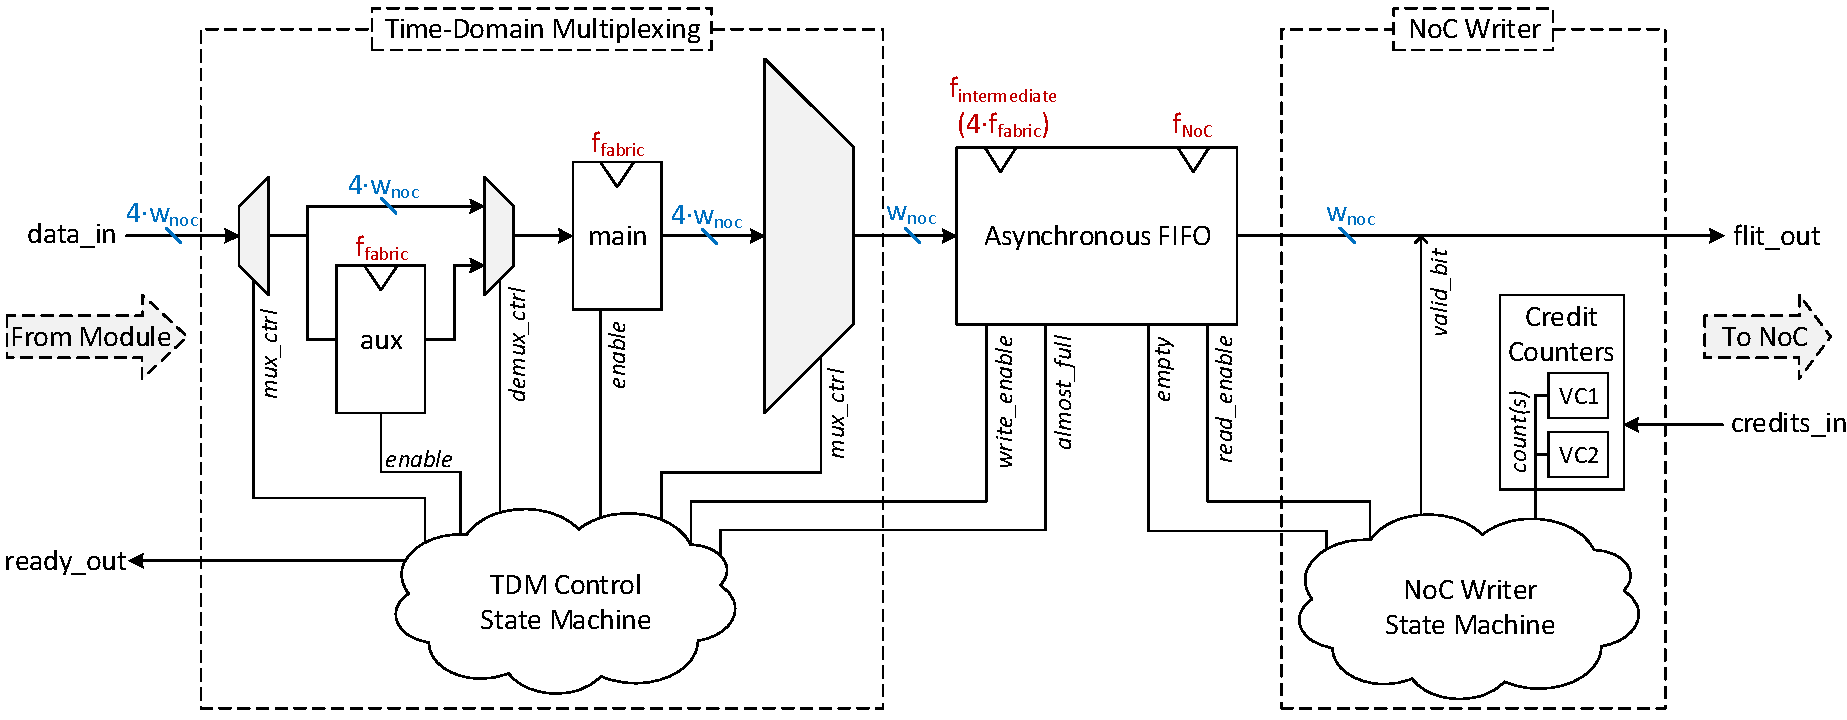
\includegraphics[width=2\columnwidth,keepaspectratio]{images/fpin_detail}
   \label{fpin}
 }
 \\
\subfloat[FabricPort output: from the embedded NoC to the FPGA fabric.]{
   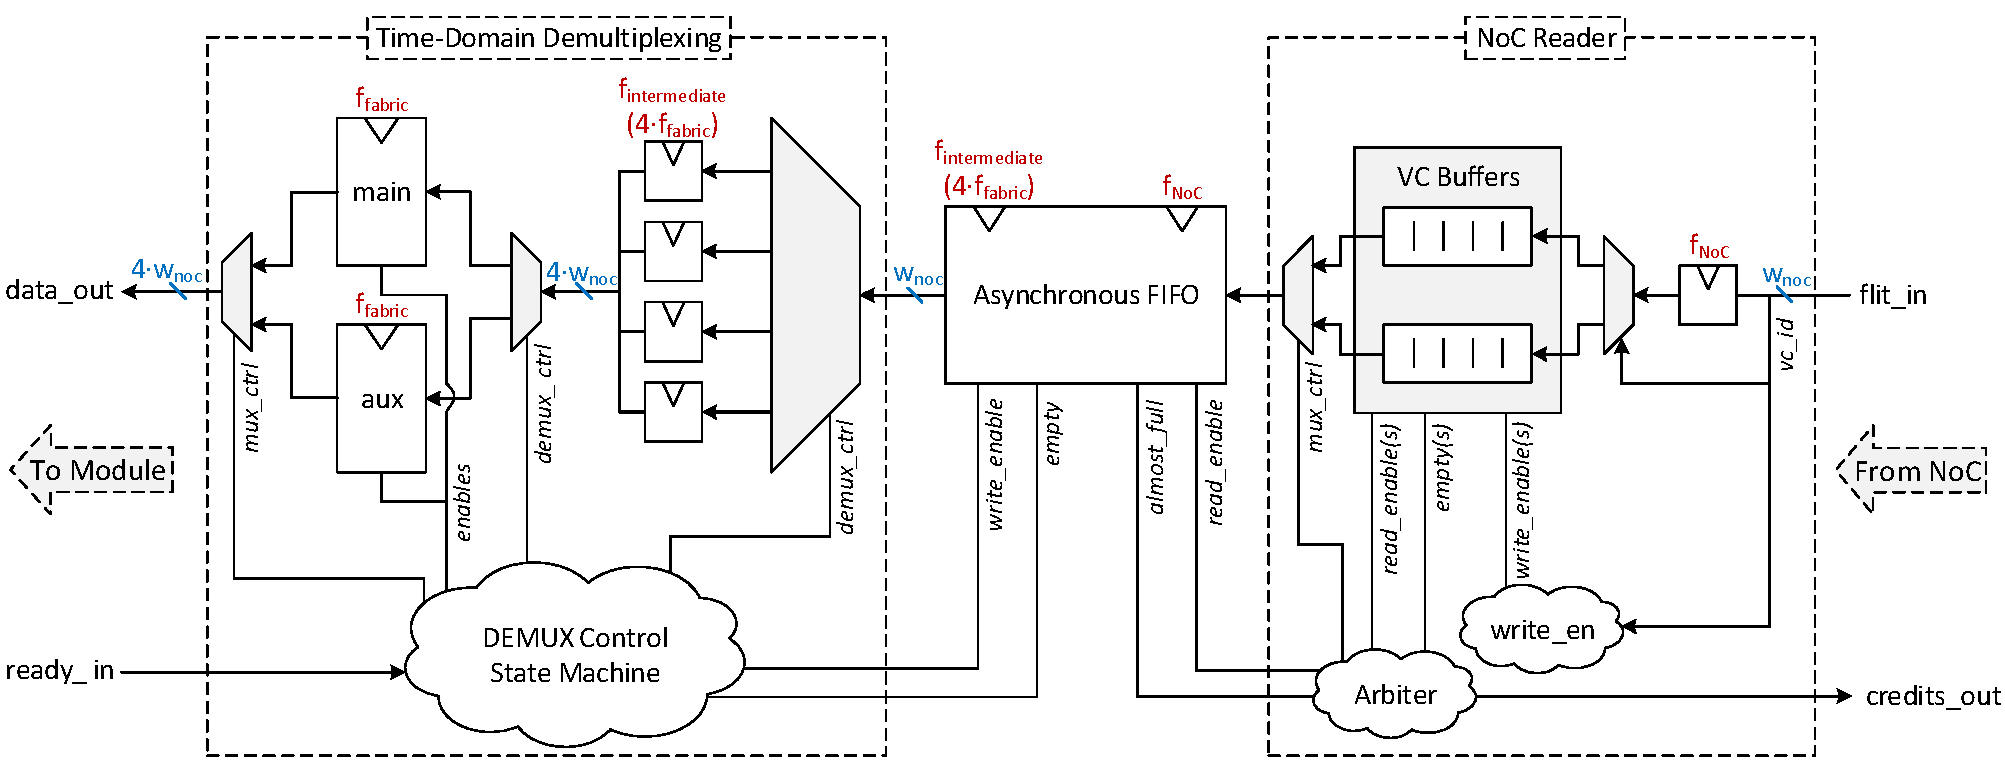
\includegraphics[width=2\columnwidth,keepaspectratio]{images/fpout_detail}
   \label{fpout}
 }
\caption{The FabricPort interfaces the FPGA fabric to an embedded NoC in a flexible way by bridging the different frequencies and widths as well as handling backpressure from both the FPGA fabric and the NoC.}
\label{fabric_port}
\end{figure*}

%----------------------------------------------------------------------------
\subsubsection{FabricPort Input: Fabric$\rightarrow$NoC}
%----------------------------------------------------------------------------

Fig.~\ref{fabric_port} shows a schematic of the FabricPort with important control signals annotated.
The FabricPort input (Fig.~\ref{fpin}) connects the output of a module in the FPGA fabric to an embedded NoC input.
Following the diagram from left to right: data is input to the time-domain multiplexing (TDM) circuitry on each fabric clock cycle and is buffered in the ``main" register.
The ``aux" register is added to provide elasticity. Whenever the output of the TDM must stall there is a clock cycle before the stall signal is processed by the fabric module. 
In that cycle, the incoming datum may still be valid, and is therefore buffered in the ``aux" registers.
To clarify this ready-valid behavior, example waveforms are illustrated in Fig.~\ref{stall_protocol}.
Importantly, this stall protocol ensures that every stall (ready = 0) cycle only stops the input for exactly one cycle ensuring that the FabricPort input does not reduce throughput.

The TDM unit takes four flits input on a slow fabric clock and outputs one flit at a time on a faster clock that is 4\xx as fast as the FPGA fabric -- we call this the intermediate clock.
This intermediate clock is only used in the FabricPort between the TDM unit and the asynchronous FIFO (aFIFO) buffer.
Because it is used only in this very localized region, this clock may be derived locally from the fabric clock by careful design of circuitry that multiplies the frequency of the clock by four.
This is better than generating 16 different clocks globally through phase-locked loops, then building a different clock tree for each router's intermediate clock (a viable but more costly alternative).

The output of the TDM unit is a new flit on each intermediate clock cycle.
Because each flit has a valid bit, only those flits that are valid will actually be written in the aFIFO thus ensuring that no invalid data propagates downstream, unnecessarily consuming power and bandwidth.
The aFIFO bridges the frequency between the intermediate clock and the NoC clock ensuring that the fabric clock can be completely independent from the NoC clock frequency and phase.

The final component in the FabricPort input is the ``NoC Writer".
This unit reads flits from the aFIFO and writes them to the downstream NoC router.
The NoC Writer keeps track of the number of credits in the downstream router to interface to the credit-based backpressure system in the embedded NoC, and only sends flits when there are available credits.
Note that credit-based flow control is by far the most-widely-used backpressure mechanism in NoCs because of its superior performance with limited buffering~\cite{dally_book}.
%Each sender keeps count of the number of credits; the sender has a credit for each available downstream buffer location.
%Therefore, a sender will only send data if it has available credits (telling it that there is buffer space downstream). 
%The downstream buffer sends a credit upstream only when it has freed one of its buffer locations by forwarding a flit.

%
%----------------------------------------------------------------------------
\subsubsection{FabricPort Output: NoC$\rightarrow$Fabric}
%----------------------------------------------------------------------------
%

Fig.~\ref{fpout} details a FabricPort output; the connection from an NoC output port to the input of a module on the FPGA fabric.
Following the diagram from right to left: the first component is the ``NoC Reader".
This unit is responsible for reading flits from an NoC router output port and writing to the aFIFO.
Note that separate FIFO queues must be kept for each VC; this is very important as it avoids scrambling data from two packets.
Fig.~\ref{demux} clarifies this point; the upstream router may interleave flits from different packets if they are on different VCs. 
By maintaining separate queues in the NoC reader, we can rearrange flits such that flits of the same packet are organized one after the other.

The NoC reader is then responsible for arbitrating between the FIFO queues and forwarding one (entire) packet -- one flit at a time -- from each VC.
We currently implement fair round-robin arbitration and make sure that there are no ``dead" arbitration cycles.
That means that as soon as the NoC reader sees a tail flit of one packet, it has already computed the VC from which it will read next.
The packet then enters the aFIFO where it crosses clock domains between the NoC clock and the intermediate clock.

The final step in the FabricPort output is the time-domain demultiplexing (DEMUX).
This unit reassembles packets (or packet fragments if a packet is longer than 4 flits) by combining 1-4 flits into the wide output port.
In doing so, the DEMUX does not combine flits of different packets and will instead insert invalid zero flits to pad the end of a packet that doesn't have a number of flits divisible by 4 (see Fig.~\ref{demux}).
%This is very much necessary to simplify the output of the NoC into something that is understandable by designers thereby creating an abstracted view of the NoC without complicating design.
This is very much necessary to present a simple interface for designers allowing them to connect design modules to the FabricPort with minimal soft logic.


%
\figvs{1}{demux}{}{``NoC Reader" sorts flits from each VC into a separate queue thereby ensuring that flits of each packet are contiguous. The DEMUX then packs up to four flits together and writes them to the wide output port but never mixes flits of two packets.}
%

%
%------------------------------------------------------------------------------------------------------------------------------
\subsection{FabricPort Discussion}
%------------------------------------------------------------------------------------------------------------------------------
%

%
%----------------------------------------------------------------------------
\subsubsection{Module Connectivity}
%----------------------------------------------------------------------------
%

The FabricPort converts 22.5~GB/s of NoC link data bandwidth (150~bits, 1.2~GHz) to 600~bits and any fabric frequency on the fabric side.
An FPGA designer can then use any fraction of that port width to send data across the NoC.
However, the smallest NoC unit is the flit; so we can either send 1, 2, 3 or 4 flits each cycle.
If the designer connects data that fits in one flit (150~bits or less), all the data transported by the NoC is useful data.
However, if the designer want to send data that fits in one-and-a-half flits (225~bits for example), then the FabricPort will send two flits, and half of the second flit is overhead that adds to power consumption and worsens NoC congestion unnecessarily.
Efficient ``translator" modules (see Fig.~\ref{fp_logical}) will therefore try to take the flit width into account when injecting data to the NoC.

\comment{
Note that the FabricPort's width is limited to 600 bits for our NoC and 20 bits of those will be used for control, leaving 580 bits for the designer to connect to their design modules.
Datapaths that are wider than 580 bits must be serialized through extra soft logic.


One clear limitation of the FabricPort is that the width is limited to 600 bits for our NoC and 20 bits of those will be used for control, leaving 580 bits for the designer to connect to their design modules.
Datapaths that are wider than 580 bits must be serialized through extra soft logic.
}


A limitation of the FabricPort output is observed when connecting two modules.
Even if each module only uses half the FabricPort's width (2 flits), only one module can receive data each cycle because the DEMUX only outputs one packet at a time by default as Fig.~\ref{demux} shows.
To overcome this limitation, we create a \textit{combine-data} mode as shown in Fig.~\ref{merge}.
For this combine-data mode, when there are two modules connected to one FabricPort, data for each module must arrive on a different VC.
The NoC Reader arbiter must strictly alternate between VCs, and then the DEMUX will be able to group two packets (one from each VC) before data output to the FPGA.
This allows merging two streams without incurring serialization latency in the FabricPort.
%
\begin{cond}
To combine packets at a FabricPort output, each packet must arrive on a different VC.
\end{cond}
%
Note that we are limited to the merging of two packets with 2 VCs but we can merge up to four 1-flit packets if we increase the number of VCs to four in the embedded NoC.
%Previous work has also identified the importance of merge functionality for FPGA applications and proposed creating NoCs out of split-merge primitives~\cite{Kapre2006}.

%
\figvs{1}{merge}{}{FabricPort output merging two packets from separate VCs in \textit{combine-data} mode, to be able to output data for two modules in the same clock cycle.}
%

%
%----------------------------------------------------------------------------
\subsubsection{Frequency and Latency}
%----------------------------------------------------------------------------
%


Fig.~\ref{zl_latency} plots the zero-load latency of the NoC (running at 1.2~GHz) for different fabric frequencies that are typical of FPGAs.
We measure latency by sending a single 4-flit packet through the FabricPort input$\rightarrow$NoC$\rightarrow$FabricPort output.
The NoC itself is running at a very fast speed, so even if each NoC hop incurs 4 cycles of NoC clocks, this translates to approximately 1 fabric clock cycle.
However, the FabricPort latency is a major portion of the total latency of data transfers on the NoC; it accounts for 40\%--85\% of latency in an unloaded embedded NoC.
The reason for this latency is the flexibility offered by the FabricPort -- we can connect a module of any operating frequency but that incurs TDM, DEMUX and clock-crossing latency.
Careful inspection of Fig.~\ref{zl_latency} reveals that the FabricPort input always has a fixed latency for a given frequency, while the latency of the FabricPort output varies by one cycle sometimes -- this is an artifact of having to wait for the \textit{next} fabric (slow) clock cycle on which we can output data in the DEMUX unit.
\comment{Additionally, the latency of the FabricPort is lowest at 300~MHz.
This is because 300~MHz is exactly one quarter of the NoC frequency, meaning that the intermediate clock is the same as the NoC clock and the aFIFO reads and writes flits at the same frequency, thus no additional clock-crossing latency is incurred.}


%
%

%
%
%#############################################################
\section{FPGA-dictated NoC Design}
\label{sec_fpganoc}
%-0-0-0-0-0-0-0-0-0-0-0-0-0-0-0-0-0-0-0-0-0-0-0-0-0-0-0-0-0-0-
%
%
%
\comment{
\begin{itemize}
	\item in cmps where all data are cache lines and there is a limited number of outstanding requests, and incoming data each has a tag to indicate which it is. processors can resolve exactly what to do with this data.
	\item we want to have streams of data so we can either tag each packet with a order id and add reordering buffers which may be huge and impossible to size, or we can constrain the NoC such that packets always arrive in-order.
	\item this means that we must use deterministic routing algorithms -- we use dor, and we can use VCs but each message class is limited to using only a single VC.
	\item give formal notation for the constraint on VCs -- data originating at a src and going to a dest must stay on the same VC.
	\item an average user should not be aware that the NoC exists: it is simply a portal in which s/he can throw data in and expect it to arrive at the other end.
	\item usually people don't care how efficiently they are actually using their interconnect resources.
	\item advanced designers will want to make best use of the NoC bandwidth/power and can therefore optimize the data size before inserting into the NoC and write custom interfaces in which case they would want to know the min flit width and min packet width -- the former is relevant for latency-insensitive and the latter is relevant for latency-sensitive.
	\item we can use the NoC both in latency-sensitive mode when we establish a permanent channel between two modules (and here we have the advantage of parallel compilation, freedom of placement etc)
	\item or latency-insensitive mode for everything else when we cannot map communication into non-intersecting paths on the NoC.
\end{itemize}
}
%
%

Fig.~\ref{classification} shows the two possibilities of synchronous design styles, as well as two communication protocols that are common in FPGA designs.
%The two design styles are ``latency-insensitive", and ``latency-sensitive". 
In a latency-insensitive system, the design consists of \textit{patient} modules that can be stalled, thus allowing the interconnect between those modules to have arbitrary delay~\cite{Carloni2002}.
Latency-sensitive design, on the other hand, does not tolerate variable latency on its connections, and assumes that its interconnect always has a fixed latency.
In this section we investigate how to map applications that belong to either design style (and any communication protocol) onto the NoC; Fig.~\ref{sys} illustrates this.
We are effectively augmenting the FPGA with a wide stallable network of buffered interconnect that can do flexible switching -- how can we best leverage that new interconnection resource for different design styles? 
And can this embedded NoC be used for both latency insensitive/sensitive design styles, and both communication protocols?

%
\figvs{1}{zl_latency}{trim = 1.7cm 2.4cm 1.7cm 2.0cm, clip}{Zero-load latency of the embedded NoC (including FabricPorts) at different fabric frequencies. Latency is reported as the number of cycles at each frequency. The number of hops varies from 1 hop (minimum) to 7 hops (maximum -- chip diagonal).}
%

%
\figvs{1}{classification}{}{Design styles and communication protocols.}
%

%
\figvs{1}{sys}{}{Mapping latency-sensitive and latency-insensitive systems onto an embedded NoC. We reserve \textit{Permapaths} on the NoC to guarantee a fixed latency and perfect throughput for a latency-sensitive application. For latency-insensitive systems, modules must be encapsulated with wrappers to add stall functionality.}
%


%
%--------------------------------------------------------------------------------------------------------
\subsection{Packet Ordering and Dependencies}
%--------------------------------------------------------------------------------------------------------
%

%
%--------------------------------------------------------------
\subsubsection{Ordering}
%--------------------------------------------------------------
%

Packet-switched NoCs like the one we are using were originally built for chip multiprocessors (CMPs).
CMPs only perform \textbf{memory-mapped} communication; most transfers are cache lines or coherency messages.
Furthermore, processors have built-in mechanisms for reordering received data, and NoCs are typically allowed to reorder packets.
%do not guarantee that packets will arrive in order.

With FPGAs, memory-mapped communication can be one of two main things: (1) Control data from a soft processor that is low-bandwidth and latency-critical -- a poor target for embedded NoCs, or (2) Communication between design modules and on-chip or off-chip memory, or PCIe links -- high bandwidth data suitable for our proposed NoC.
Additionally, FPGAs are very good at implementing \textbf{streaming}, or data-flow applications such as packet switching, video processing, compression and encryption.
These streams of data are also prime targets for using our high-bandwidth embedded NoC.
Crucially, neither memory-mapped nor streaming applications tolerate packet reordering on FPGAs, nor do FPGAs natively support it.
While it may be possible to design reordering logic for simple memory-mapped applications, it becomes \textit{impossible} to build such logic for streaming applications without hurting performance -- we therefore choose to restrict the embedded NoC to perform in-order data transfers only.
Specifically, an NoC is not allowed to reorder packets on a single connection.
%
\begin{defn}
A \textbf{connection} (\textbf{s}, \textbf{d}) exists between a single source (\textbf{s}) and its downstream destination (\textbf{d}) to which it sends data.
\end{defn}
%
\begin{defn}
A \textbf{path} is the sequence of links from \textbf{s} to \textbf{d} that a flit takes in traversing an NoC.
\end{defn}
%

There are two causes of packet reordering.
Firstly, an adaptive route-selection algorithm would always attempt to choose a path of least contention through the NoC; therefore two packets of the same source and destination (same connection) may take different paths and arrive out of order.
Secondly, when sending packets (on the same connection) but different VCs, two packets may get reordered even if they are both taking the same path through the NoC.

To solve the first problem, we only use routing algorithms, in which routes are the same for all packets that belong to a connection.
%
\begin{cond}
\label{routing_constraint}
The same \textbf{path} must be taken by all packets that belong to the same \textbf{connection}.
\end{cond}
%
%
Deterministic routing algorithms such as dimension-ordered routing~\cite{dally_book} fulfill Condition~\ref{routing_constraint} as they always select the same route for packets on the same connection.
%


Eliminating VCs altogether would fix the second ordering problem; however, this is not necessary.
VCs can be used to break message deadlock, merge data streams (Fig.~\ref{merge}), alleviate NoC congestion and may be also used to assign packet priorities thus adding extra configurability to our NoC -- these properties are desirable.
We therefore impose more specific constraints on VCs such that they may still be used on FPGA NoCs.
%
\begin{cond}
All packets belonging to the same \textbf{connection} must use the same VC.
\end{cond}
%


To do this in NoC routers is simple.
Normally, a packet may change VCs at every router hop -- VC selection is done in a VC allocator~\cite{dally_book}.
We replace this VC allocator with a lightweight VC \textit{facilitator} that cannot switch a packet between VCs; instead, it inspects a packet's input VC and stalls that packet until the downstream VC buffer is available.
At the same time, other connections may use other VCs in that router thus taking advantage of multiple VCs.


%
%--------------------------------------------------------------
\subsubsection{Dependencies and Deadlock}
%--------------------------------------------------------------
%

\begin{figure}[t]
\centering
\subfloat[Standard FabricPort output.]{
   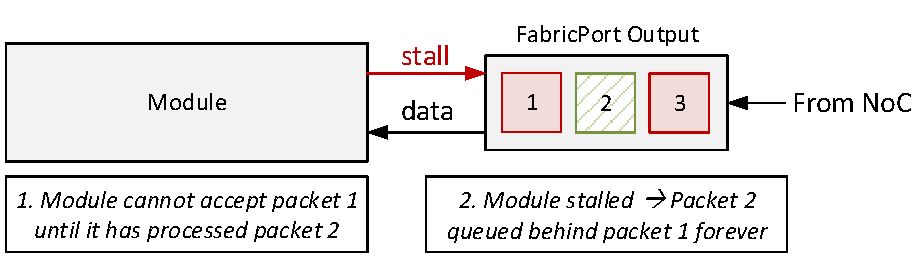
\includegraphics[width=0.9\columnwidth,keepaspectratio]{images/deadlock}
   \label{deadlock}
 }
 \\
\subfloat[Deadlock-free FabricPort output.]{
   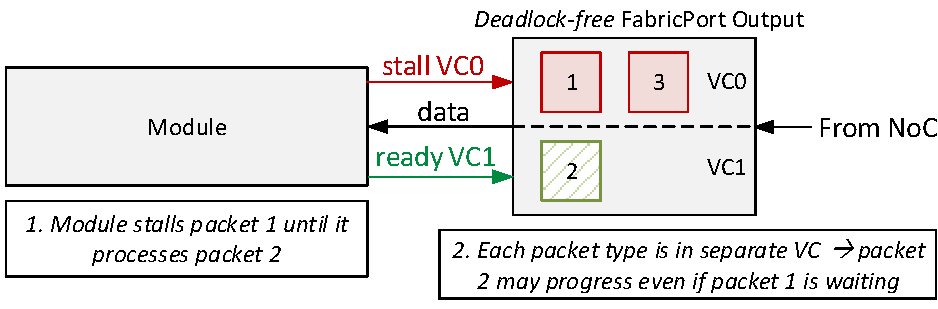
\includegraphics[width=0.9\columnwidth,keepaspectratio]{images/nodeadlock}
   \label{nodeadlock}
 }
\caption{Deadlock can occur if a dependency exists between two message types going to the same port. By using separate VCs for each message type, this deadlock can be broken thus allowing two dependent message types to share a FabricPort output.}
\label{dead}
\end{figure}


Two \textit{message types} may not share a standard FabricPort output (Fig.~\ref{fpout}) if a dependency exists between the two message types.
An example of dependent message types can be seen in video processing IP cores: both control messages (that configure the IP to the correct resolution for example) and data messages (pixels of a video stream) are received on the same port~\cite{altera_vip}.
An IP core may not be able to process the data messages correctly until it receives a control message.

Consider the deadlock scenario in Fig.~\ref{deadlock}.
The module is expecting to receive packet 2 but gets packet 1 instead; therefore it stalls the FabricPort output and packet 2 remains queued behind packet 1 forever.
To avoid this deadlock, we can send each message type in a different VC~\cite{Sorin2011}.
Additionally, we created a deadlock-free FabricPort output that maintains separate paths for each VC -- this means we duplicate the aFIFO and DEMUX units for each VC we have.
There are now two separate ``ready" signals; one for each VC, but there is still only one data bus feeding the module. 
The module can therefore \textit{either} read from VC0 or VC1.
Fig.~\ref{nodeadlock} shows that even if there is a dependency between different messages, they can share a FabricPort output provided each uses a different VC.
%
\begin{cond}
When multiple message types can be sent to a FabricPort, and a dependency exists between the message types, each type must use a different VC.
\end{cond}
%

%
%---------------------------------------------------------------------------------------------------------
\subsection{Latency-Insensitive Design with NoC}
%---------------------------------------------------------------------------------------------------------
%

Latency-insensitive design is a design methodology that decouples design modules from their interconnect by forcing each module to be \textit{patient}; that is, to tolerate variable latency on its inputs~\cite{Carloni2002}.
This is typically done by encapsulating design modules with wrappers that can stall a module until its input data arrives.
This means that a design remains functionally correct, by construction, regardless of the latency of data arriving at each module.
The consequence of this latency tolerance is that a CAD tool can automatically add pipeline stages (called \textit{relay stations}) invisibly to the circuit designer, late in the design compilation and thus improve frequency without extra effort from the designer~\cite{Carloni2002}.

Our embedded NoC is effectively a form of latency-insensitive interconnect; it is heavily pipelined and buffered and supports stalling.
We can therefore leverage such an NoC to interconnect patient modules of a latency-insensitive system as illustrated in Fig.~\ref{sys}. 
Furthermore, we no longer need to add relay stations on connections that are mapped to NoC links, avoiding their overhead.

%
\figvs{0.96}{li_wrappers_overhead}{trim = 1.5cm 3.7cm 1.5cm 3.45cm, clip}{Area and frequency of latency-insensitive wrappers from~\cite{Murray2014} (original), and optimized wrappers that take advantage of NoC buffering (NoC-compatible).}
%

Previous work that investigated the overhead of latency-insensitive design on FPGAs used FIFOs at the inputs of modules in the stall-wrappers to avoid throughput degradation whenever a stall occurs~\cite{Murray2014}.
When the interconnect is an embedded NoC; however, we already have sufficient buffering in the NoC itself (and the FabricPorts) to avoid this throughput degradation, thus allowing us to replace this FIFO -- which is a major portion of the wrapper area -- by a single stage of registers.
We compare the area and frequency of the original latency-insensitive wrappers evaluated in~\cite{Murray2014}, and the NoC-compatible wrappers in Fig.~\ref{li_wrappers_overhead} for wrappers that support one input and one output and a width between 100 bits and 600 bits.
As Fig.~\ref{li_wrappers_overhead} shows, the lightweight NoC-compatible wrappers are 87\% smaller and 47\% faster.

We envision a future latency-insensitive design flow targeting embedded NoCs on FPGAs.
Given a set of modules that make up an application, they would first be encapsulated with wrappers, then mapped onto an NoC such that performance of the system is maximized.


%
%---------------------------------------------------------------------------------------------------------
\subsection{Latency-Sensitive Design with NoC\\(Permapaths)}
%---------------------------------------------------------------------------------------------------------
%

%need to introduce latency insensitive design
Latency-sensitive design requires predictable latency on the connections between modules.
That means that the interconnect is not allowed to insert/remove any cycles between successive data.
Prior NoC literature has largely focused on using circuit-switching to achieve quality-of-service guarantees but could only provide a bound on latency rather than a guarantee of fixed latency~\cite{Goossens2005}.
We analyze the latency and throughput guarantees that can be attained from an NoC, and use those guarantees to determine the conditions under which a latency-sensitive system can be mapped onto a packet-switched embedded NoC.
Effectively, our methodology creates permanent paths with predictable latencies (Permapaths) on our packet-switched embedded NoC.

%
%----------------------------------------------------------------------------
\subsubsection{Latency and Throughput Guarantees}
\label{subsec_guarantees}
%----------------------------------------------------------------------------
%


To ensure that the NoC doesn't stall due to unavailable buffering, we size NoC buffers for maximum throughput, so that we never stall while waiting for backpressure signals within the NoC.
This is well-studied in the literature and is done by sizing our router buffers to cover the \textit{credit round-trip latency}~\cite{dally_book} -- for our system, a buffer depth of 10 suffices.



Fig.~\ref{zl_xput} plots the throughput between any source and destination on our NoC in the absence of contention.
The NoC is running at 1.2~GHz with 1-flit width; therefore, if we send 1 flit each cycle at a frequency lower than 1.2~GHz, our throughput is always perfect -- we'll receive data at the same input rate (one flit per cycle) on the other end of the NoC path. 
In fact, the NoC connection acts as a simple pipelined wire; the number of pipeline stages are equivalent to the zero-load latency of an NoC path; however, it is irrelevant because that latency is only incurred once at the very beginning of data transmission after which data arrives on each fabric clock cycle.
We call this a \textbf{Permapath} through the NoC: a path that is free of contention and has perfect throughput.
As Fig.~\ref{zl_xput} shows, we can create Permapaths of larger widths provided that the input bandwidth of our connection does not exceed the NoC port bandwidth of 22.5~GB/s.
This is why throughput is still perfect with 4~flits$\times$300~MHz for instance.
To create those Permapaths we must therefore ensure two things:
%
\begin{cond}
(Permapaths)
The sending module data bandwidth must be less than or equal to the maximum FabricPort input bandwidth.
\end{cond}
%
\begin{cond}
\label{traf_cond}
(Permapaths)
No other data traffic may overlap the NoC links reserved for a Permapath to avoid congestion delays on those links.
\end{cond}
%
Condition~\ref{traf_cond} be determined statically since our routing algorithm is deterministic; therefore, the mapping of modules onto NoC routers is sufficient to identify which NoC links will be used by each module.


%
\figvs{0.96}{zl_xput}{trim = 1.5cm 3.7cm 1.5cm 3.45cm, clip}{Zero-load throughput of embedded NoC path between any two nodes, normalized to sent data. A throughput of ``1" is the maximum; it means that we receive $i$ flits per cycle, where $i$ is the number of flits we insert in the FabricPort each cycle.}
%

%
%---------------------------------------------------------------------------------------------------------
\subsection{Multicast, Reconvergence and Feedback}
%---------------------------------------------------------------------------------------------------------
%

%
\figvs{0.8}{multicast}{}{Aspects of complex FPGA applications.}
%

A complex FPGA application may include multicast, reconvergence and feedback as shown in Fig.~\ref{multicast} -- we discuss these aspects briefly here but leave the in-depth analysis for future work.
Prior NoC research has shown that packet-switched routers can be augmented with multicast capability at very low area overhead~\cite{Enright2008}.
As for reconvergence, the two branches of a reconvergent path may have different latencies on the embedded NoC with different implications for latency-sensitive and latency-insensitive systems.
A latency-sensitive system may become functionally incorrect in that case; the designer must therefore ensure that the paths are balanced.
For a latency-insensitive system functional correctness is guaranteed but throughput degradation may occur if latencies of the two paths differ by a large amount; prior work has investigated path balancing for latency-insensitive systems~\cite{Lu2003}.
Balancing can be done by selecting two paths of the same length through the NoC (hence same latency) and using registers in the FPGA fabric for fine-grained latency adjustment.
Feedback paths are also tricky to implement on embedded NoCs; this stems from the fact that these connections are typically latency-critical and require very low latency so as not to impede throughput.

While some of these connections can be mapped onto the NoC, not all of them have to be; the embedded NoC is not meant to be an interconnect capable of connecting everything on the FPGA; rather a flexible low-cost (but high bandwidth) interconnect resource that \textit{augments} the current FPGA traditional interconnect. 
Remember that the embedded NoC is 1.3\% of FPGA core area while the FPGA's traditional interconnect accounts for \til50\%~\cite{Lewis2013}.
Traditional interconnect can still be used for latency-critical connections while the embedded NoC can be leveraged for connections on which timing closure is difficult or those that require buffering, stallability, or heavy switching.



%
%

%
%
%#############################################################
%\section{Simulator}
%-0-0-0-0-0-0-0-0-0-0-0-0-0-0-0-0-0-0-0-0-0-0-0-0-0-0-0-0-0-0-
%
%%
%
\comment{
\begin{itemize}
	\item flexible simulator that interfaces modelsim to booksim so we can model any NoC we want on the booksim side and any design we want on modelsim side and still get cycle-accurate results.
	\item interface sends flits and credits
	\item uses systemverilog dpi interface and unix sockets to communicate between the two programs
\end{itemize}
}
%
%

To evaluate the performance of embedded NoCs, we created \texttt{RTL2Booksim}\footnote{\texttt{RTL2Booksim} is available for download at \\\url{www.eecg.utoronto.ca/~mohamed/rtl2booksim.html}}: a simulation framework which allows the co-simulation of hardware description languages (HDL) such as Verilog and VHDL, and a widely-used cycle-accurate NoC simulator called Booksim~\cite{booksim}.


%
%

%
%
%#############################################################
\section{Application Case Studies}
\label{sec_apps}
%-0-0-0-0-0-0-0-0-0-0-0-0-0-0-0-0-0-0-0-0-0-0-0-0-0-0-0-0-0-0-
%
\subsection{Simulator}
\label{sec:sim}
%
%
\comment{
\begin{itemize}
	\item flexible simulator that interfaces modelsim to booksim so we can model any NoC we want on the booksim side and any design we want on modelsim side and still get cycle-accurate results.
	\item interface sends flits and credits
	\item uses systemverilog dpi interface and unix sockets to communicate between the two programs
\end{itemize}
}
%
%

To evaluate the performance of embedded NoCs, we created \texttt{RTL2Booksim}\footnote{\texttt{RTL2Booksim} is available for download at \\\url{www.eecg.utoronto.ca/~mohamed/rtl2booksim.html}}: a simulation framework which allows the co-simulation of hardware description languages (HDL) such as Verilog and VHDL, and a widely-used cycle-accurate NoC simulator called Booksim~\cite{booksim}.


%
%

%
\subsection{JPEG Compression\\\textit{(Latency-sensitive, streaming)}}
%
%
\comment{
\begin{itemize}
	\item look at jpeg compression for instance -- conforms to our constraints for a design that can map latency-sensitively onto the NoC
	\item establish communication channels and data arrives each cycle -- we don't even need the ready signals
	\item what advantages does this bring? lets try placing the modules connecting to the routers or connecting together
	\item how much global interconnect does it save?
	\item present a simple cad algo to say whether this app can be mapped latency-sensitvely or not? and give candidate solutions if possible
\end{itemize}
}
%---------------------------------------------------------------------------------------------------------------------------------------------------

%
\figvs{1}{jpeg_app}{}{Single-stream JPEG block diagram.}
%

We use a streaming JPEG compression design from~\cite{jpeg_opencore}.
The application consists of three modules as shown in Fig.~\ref{jpeg_app}; discrete cosine transform (DCT), quantizer (QNR) and run-length encoding (RLE).
The single pipeline shown in Fig.~\ref{jpeg_app} can accept one pixel per cycle and a data strobe that indicates the start of 64 consecutive pixels forming one (8$\times$8) block on which the algorithm operates~\cite{jpeg_opencore}.
The components of this system are therefore latency-sensitive as they rely on pixels arriving every cycle, and the modules do not respond to backpressure.

We parallelize this application by instantiating multiple (10--40) JPEG pipelines in parallel; which means that the connection width between the DCT, QNR and RLE modules varies between 130~bits and 520~bits.
Parallel JPEG compression is an important data-center application as multiple images are often required to be compressed at multiple resolutions before being stored in data-center disk drives; the back-end of large social networking websites and search engines.
We implemented this parallel JPEG application using direct point-to-point links, then mapped the same design to use the embedded NoC between the modules using \textbf{Permapaths} similarly to Fig.~\ref{sys}.
Using the \texttt{RTL2Booksim} simulator, we connected the JPEG design modules through the FabricPorts to the embedded NoC and verified functional correctness of the NoC-based JPEG.
Additionally, we verified that throughput (in number of cycles) was the same for both the original and NoC versions; however, there are \til8 wasted cycles (equivalent to the zero-load latency of three hops) at the very beginning in the NoC version while the NoC link pipeline is getting populated with valid output data -- these 8 cycles are of no consequence.

%---------------------------------------------------------------------------------------
\subsubsection{Frequency}
%---------------------------------------------------------------------------------------

To model the physical design repercussions (placement, routing, critical path delay) of using an embedded NoC, we emulated embedded NoC routers on FPGAs by creating 16 design partitions in Quartus~II that are of size 7$\times$5$=$35 logic clusters -- each one of those partitions represents an embedded hard NoC router with its FabricPorts and interface to FPGA (see Fig.~\ref{heat_map} for chip plan).
We then connected the JPEG design modules to this emulated NoC.
Additionally, we varied the physical location of the QNR and RLE modules (through location constraints) from ``close" together on the FPGA chip to ``far" on opposite ends of the chip.
Note that the DCT module wasn't placed in a partition as it was a very large module and used most of the FPGA's DSP blocks.

%
\figvs{1}{jpeg_freq}{trim = 1.5cm 3.7cm 1.5cm 3.45cm, clip}{Frequency of the parallel JPEG compression application with and without an NoC. The plot ``with NoC" is averaged for the two cases when it's ``close" and ``far" with the standard deviation plotted as error bars. Results are averaged over 3 seeds.}
%

Using location constraints, we investigated the result of a stretched critical path in an FPGA application.
This could occur if the FPGA is highly utilized and it is difficult for the CAD tools to optimize the critical path as its endpoints are forced to be placed far apart, or when application modules connect to I/O interfaces and are therefore physically constrained far from one another.
Fig.~\ref{jpeg_freq} plots the frequency of the original parallel JPEG and the NoC version.
In the ``close" configuration, the  frequency of the original JPEG is higher than that of the NoC version by \til5\%. 
This is because the JPEG pipeline is well-suited to the FPGA's traditional row/column interconnect.
With the NoC version, the wide point-to-point links must be connected to the smaller area of 7$\times$5 logic clusters (area of an embedded router); making the placement less regular and on average slightly lengthening the critical path.

%
\figvs{1}{jpeg_pipes}{trim = 1.5cm 3.3cm 1.5cm 3.77cm, clip}{Frequency of parallel JPEG with 40 streams when we add 1-4 pipeline stages on the critical path. Frequency of the same application when connected to the NoC is plotted for comparison. Results are averaged over 3 seeds.}
%

The advantage of the NoC is highlighted in the ``far" configuration when the QNR and RLE modules are placed far apart thus stretching the critical path across the chip diagonal.
In the NoC version, we connect to the closest NoC router as shown in Fig.~\ref{heat_map} -- on average, the frequency improved by \til80\%.
Whether in the ``far" or ``close" setups, the NoC-version's frequency only varies by \til6\% as the error bars show in Fig.~\ref{jpeg_freq}.
By relying on the NoC's predictable frequency in connecting modules together, the effects of the FPGA's utilization level and the modules' physical placement constraints become localized to each module instead of being a global effect over the entire design.
Modules connected through the NoC become timing-independent making for an easier CAD problem and allowing parallel compilation.


With additional design effort, a designer of the original (without NoC) system would identify the critical path and attempt to pipeline it so as to improve the design's frequency.
This design$\rightarrow$compile$\rightarrow$repipeline cycle hurts designer productivity as it can be unpredictable and compilation could take days for a large design~\cite{Murray2014}.
We plot the frequency of our original JPEG with 40 streams in the ``far" configuration after adding 1, 2, 3, and 4 pipeline registers on the critical path, both with and without register retiming optimizations, and we compare to the NoC version frequency in Fig.~\ref{jpeg_pipes}.
The plot shows that the frequency of the pipelined version never becomes as good as that of the NoC version even with 4 pipeline stages -- the NoC version is 10\% better than original JPEG with pipelining.

\comment{
The plot shows two things.
First, the frequency of the pipelined version never becomes as good as that of the NoC version even with 4 pipeline stages on the critical path -- on average, there is a 10\% difference in frequency.
Secondly, It doesn't really matter how many pipeline registers we place on the critical path, nor does it matter much whether register retiming is enabled. 
This is because register retiming occurs before placement and routing in the CAD flow, and therefore has no physical awareness on where the register will actually be placed on the FPGA device.
}


%---------------------------------------------------------------------------------------
\subsubsection{Interconnect Utilization}
%---------------------------------------------------------------------------------------

%
\begin{table}[!t]
\centering
\begin{small}
    \caption{Interconnect utilization for JPEG with 40 streams in ``far" configuration. Relative difference between NoC version and the original version is reported.}
    \label{wire_util}
    \begin{tabular}{cccc}
    \toprule
    \multicolumn{2}{c}{Interconnect Resource}       & Difference & Geomean \\
    \midrule
	\multirow{2}{*}{Short}   & Vertical (C4)         & +13.2\%   & \multirow{2}{*}{+10.2\%} \\
	                         & Horizontal (R3,R6)   & +7.8\% & \\
	\midrule
	\multirow{2}{*}{Long} & Vertical (C14)           & -47.2\% & \multirow{2}{*}{-38.6\%}\\
	& Horizontal (R24)                              & -31.6\%  & \\
    \bottomrule
	\end{tabular}
    \begin{tabular}{cccc}
	\multicolumn{4}{c}{Wire naming convention: C=column, R=row, }\\
	\multicolumn{4}{c}{followed by number of logic clusters of wire length.}\\
    \end{tabular}
\end{small}
\end{table}
%

Table~\ref{wire_util} quantifies the FPGA interconnect utilization difference for the two versions of 40-stream ``far" JPEG.
The NoC version reduces long wire utilization by \til40\% but increases short wire utilization by \til10\%.
Note that long wires are scarce on FPGAs, for the Stratix~V device we use, there are 25\xx more short wires than there are long wires.
By offloading long connections onto an NoC, we conserve much of the valuable long wires.

%
\figvs{1}{heat_map}{}{Heat map showing total wire utilization for the NoC version, and only long-wire utilization for the original version of the JPEG application with 40 streams when modules are spaced out in the ``far" configuration. In hot spots, utilization of scarce long wires in the original version goes up to 100\%, while total wire utilization never exceeds 40\% for the NoC version.}
%

Fig.~\ref{heat_map} shows wire utilization for the two versions of 40-stream ``far" JPEG and highlights that using the NoC does not produce any routing hot spots around the embedded routers.
As the heat map shows, FPGA interconnect utilization does not exceed 40\% in that case.
Conversely, the original version utilizes long wires heavily on the long connection between QNR$\rightarrow$RLE, with utilization going up to 100\% in hot spots at the terminals of the long connection as shown in Fig.~\ref{heat_map}.


%
%
%
\subsection{Ethernet Switch \textit{(Latency-insensitive, streaming)}}
%
%
%\begin{itemize}
%	\item performance of a packet-switching fabric using the NoC -- different topologies, includes interface
%\end{itemize}
%
%

%\subsubsection{Design}

%Packet switching applications switch data that has been separated into packets.
%These packets include control information that describe various attributes of the payload, such as its source and destination.
%Unlike other data streaming applications, the distribution of packet sources and destinations can vary widely, and are rarely known before runtime.
%A Ethernet switch must be capable of completing packet transmission under any possible traffic condition.

\begin{figure*}[t] \centering \vspace{0cm}
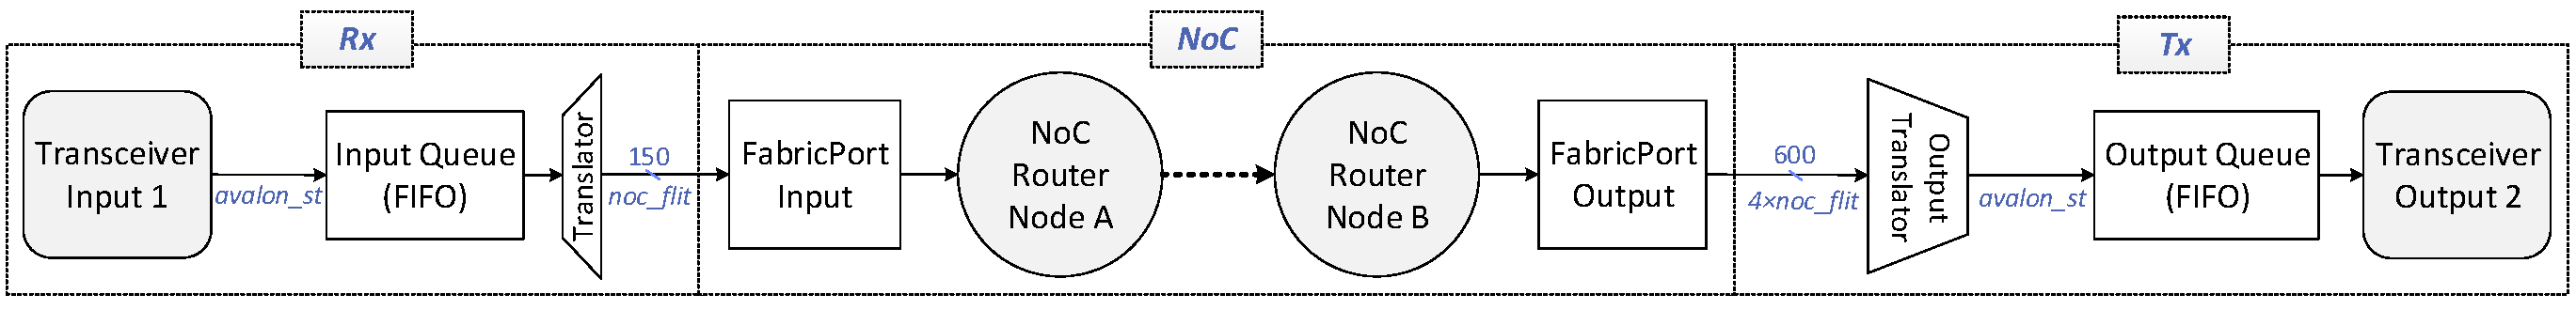
\includegraphics[width=0.95\textwidth, trim = 0cm 0.15cm 0cm 0.3cm]{images/complete-switch-path-new.pdf}
\caption{Functional block diagram of one path through our NoC Ethernet switch.}
\label{fig:switch-blk-diagram}
\vspace{0cm}
\end{figure*}


%
%\figvs{0.9}{ethernet}{}{Block diagram of NoC-based Ethernet switch.}
%

One of the most important and prevalent building blocks of communication networks is the Ethernet switch.
The embedded NoC provides a natural back-bone for an Ethernet switch design, as it includes (1) switching and (2) buffering within the NoC routers, and (3) a built-in backpressure mechanism for flow control.
Recent work has revealed that an Ethernet switch achieves significant area and performance improvements when it leverages an NoC-enhanced FPGA~\cite{Bitar2014}.
We describe here how such an Ethernet switch can take full advantage of the embedded NoC, while demonstrating that it considerably outperforms the best previously proposed FPGA switch fabric design~\cite{dai-zhu}.

%The NoC provides two possible design options for transporting packetized data, as listed below.
%We will refer to the streaming data packets as ``stream packets'' in order to avoid confusion with the NoC's packets.
%
%\begin{enumerate}
%
%\item \textbf{Encapsulate} each stream packet into multiple NoC packets.
%A NoC packet holds one data beat from the stream packet, including both payload and all control information.
%The stream packet's control data does not need to be read.
%
%\item \textbf{Translate} each stream packet into a single NoC packet.
%The stream packet's start-of-packet (SOP) and end-of-packet (EOP) data beats are sent in the head and tail flits of the NoC packet, respectively.
%Thus, the SOP and EOP signals are stripped from the stream packet before being sent through the NoC.
%
%\end{enumerate}
%
%Encapsulating the data is the simplest design option, as it only requires logic to read the data's destination before sending it through the NoC.
%Additionally, since it breaks up stream packets into smaller, fixed-size NoC packets, it can potentially achieve better latency.
%However, this design method comes with several limitations.
%Breaking packets up into smaller units introduces the possibility of packet re-ordering and packet interleaving in the NoC.
%%A centralized scheduler, similar to ones used in other Ethernet switch designs, would be needed to prevent this from occurring.
%To remedy this, each NoC packet would need additional control data indicating the flit ID and source, as well as complex re-ordering logic at the output.
%On the other hand, translating each stream packet to a NoC packet prevents packet re-ordering/interleaving, thus removing this complexity.
%Although translation requires some additional logic to perform the conversion from stream packet to NoC packet, and vice versa, this logic is far simpler than the re-ordering logic necessary for encapsulation.
%Thus, we recommend that Ethernet switch designs translate, rather than encapsulate, stream packets into NoC packets.
%%By building and simulating this design, we show that it better leverages the NoC for packet-switching applications.

%\begin{figure}[t] \centering \vspace{0cm}
%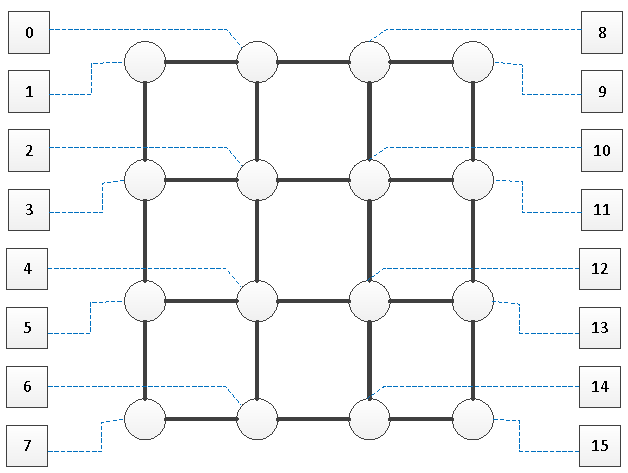
\includegraphics[width=0.4\textwidth]{images/16-node-mesh.pdf}
%\caption{Each of the 16 transceiver nodes (squares) connect to a unique NoC router (circles) through the FPGA's fabric (dashed lines)}
%\label{fig:16mesh}
%\vspace{0cm}
%\end{figure}

%Our design consists of a 16$\times$16 10-Gigabit Ethernet switch.
The embedded NoC is used in place of the switch's crossbar.
For a 16$\times$16 switch, each of the 16 transceiver nodes are connected to one of the 16 NoC routers via the FPGA's soft fabric.
%To transport 10~Gb/s data, the soft fabric is set to run at 156.25 MHz for 64-bit wide data.
%Each transceiver-to-router path consists of buffering and logic to convert stream packets to NoC packets, and vice-versa.
%The transceiver-to-router paths complete the flow shown in Fig.~\ref{fig:switch-blk-diagram}.
Fig.~\ref{fig:switch-blk-diagram} shows the path between transceiver 1 and transceiver 2; in our 16$\times$16 switch there are 256 such paths from each input to each output.
%On the receive path (\textit{Rx}), two stream flits (\textit{avalon\textunderscore st}) are joined together (\textit{2$\times$avalon\textunderscore st}) before being inserted into an input queue.
On the receive path (\textit{Rx}), Ethernet data is packed into NoC flits before being brought to the FabricPort input.
The translator sets NoC control bits such that one NoC packet corresponds to one Ethernet frame.
For example, a 512-byte Ethernet frame is converted into 32 NoC flits.
%If the NoC router's input fabric port is ready to accept data, the input queue ejects flits to the translator, which adds the necessary NoC control bits and strips the unnecessary Avalon Stream control bits (valid, SOP, EOP) before injecting the newly-created NoC flit into the fabric port.
After the NoC receives the flit from the FabricPort, it steers the flit to its destination, using dimension-order XY routing.
%\footnote{The impact of routing algorithms on NoC-based Ethernet switch performance was investigated by Bitar \textit{et al.}~\cite{Bitar2014}.}
%On the transmit path (\textit{Tx}), round-robin arbitration logic is needed, as the FabricPort can output up to four NoC flits from the same packet in the same cycle (see Section~\ref{sec_fabricport}).
%On the transmit path (\textit{Tx}), the translator uses demultiplexing in order to convert the FabricPort output width (600~bits) to the output queue width (150~bits).
On the transmit path (\textit{Tx}), the NoC can output up to four flits (600~bits) from a packet in a single system clock cycle -- this is demultiplexed in the output translator to the output queue width (150~bits).
This demultiplexing accounts for most of the translators' area in Table~\ref{tbl:hcost}.
The translator also strips away the NoC control bits before inserting the Ethernet data into the output queue.
%The output queue waits for an end-of-packet signal before beginning transmission.
%Although we set the queue size to be 64 bits wide and 512 words deep, this can be varied depending on the needs of the switch's particular application.

We synthesized the soft logic on a Stratix~V device, and
The design is synthesized on a Stratix V device and show the resource utilization in Table~\ref{tbl:hcost}.
Because we take advantage of the NoC's switching and buffering our switch is \til3$\times$ more area efficient than previous FPGA Ethernet switches~\cite{dai-zhu} even when accounting for the complete embedded NoC area.

%The buffering mechanism used by our switch is considered combined input/output queued (CIOQ).
%However, our Ethernet switch has important differences from previously proposed CIOQ architectures~\cite{minkenberg2000combined}.
%The NoC already provides built-in flow control for handling data being sent from multiple sources to a single destination.
%Thus, no centralized scheduling logic or additional flow control signals between the inputs and outputs are necessary, resulting in significant complexity savings.
%%This would not have been possible if the design had encapsulated rather than translated the data, as centralized scheduling logic would have been necessary to
%Additionally, the NoC mitigates head-of-line blocking (HOL) by buffering packets within the NoC rather than within the input queues.
%Typically, CIOQ architectures use virtual output queues (VOQ) to mitigate HOL~\cite{minkenberg2000combined}, thus revealing additional hardware cost savings for our NoC-based Ethernet switch design.

% --> Only talk about the replacement of scheduling logic by NoC backpressuring. Leave HoL discussion to journal paper?

%\begin{itemize}
%
%\item \textbf{No scheduling logic.} In nearly all Ethernet switch designs, scheduling logic is necessary to control which inputs are granted access to the switch crossbar.
%
%\item \textbf{No head-of-line blocking (HOL).}
%
%\end{itemize}

% introduce concept of translating data packets to NoC packets along with both options
% describe design (with block diagram) for 16x16 10~Gb/s
% illustrate inherent benefits of this switch: no centralized scheduler needed, no VOQs needed for HOL

%\subsubsection{Evaluation}

Two important performance metrics for Ethernet switch design are bandwidth and latency~\cite{elhanany2005network}.
The bandwidth of our NoC-based Ethernet switch is limited by the supported bandwidth of the embedded NoC.
As described in Section~\ref{sec:hnoc}, the NoC's links have a bandwidth capacity of 22.5 GB/s (180~Gb/s).
Since some of this bandwidth is used to transport packet control information, the NoC's links can support up to 153.6~Gb/s of Ethernet data.
%The worst case traffic pattern that the NoC-crossbar must support is the pattern that places the highest demand on a NoC link while driving the NoC's sinks at no higher than the line rate, $R$ ($R = 10$~Gb/s in our design).
%Analysis of the 16-node mesh reveals that the maximum NoC channel load is $3R$.
%Thus, the maximum supported bandwidth per node for our Ethernet switch is $R = 51.2$~Gb/s, or an aggregate bandwidth of 819.2~Gb/s.
Analysis of the worst case traffic in a 16-node mesh shows that the NoC can support a line rate of one third its link capacity, i.e. 51.2~Gb/s~\cite{Bitar2014}.
While previous work on FPGA switch design has achieved up to 160~Gb/s of aggregate bandwidth~\cite{dai-zhu}, our switch design can achieve 51.2$\times$16 = 819.2~Gb/s by leveraging the embedded NoC.
We have therefore implemented a programmable Ethernet switch with 16 inputs/outputs that is capable of either 10~Gb/s, 25~Gb/s or 40~Gb/s -- three widely used Ethernet standards.

%
%
\begin{table}[!t]
\centering
\begin{small}
    \caption{Hardware cost breakdown of an NoC-based 10-Gb Ethernet switch on a Stratix V device.}
    \label{tbl:hcost}
    \begin{tabular}{ccccccc}
    \toprule
     & 10GbE & I/O & Translators & \textbf{Total} \\
     & MACs & Queues &  & & \\
    \midrule
	ALMs & 24000  & 3707 &  3504 & \textbf{31211} \\
	%ALUTs & 32016 & 5616 & 2352 & \textbf{41648} \\
	%Regs  & 49232 & 3264 & 17840 & \textbf{53696} \\
	M20Ks & 0    & 192   & 0 & \textbf{192}   \\
    \bottomrule
    \end{tabular}
\end{small}
\end{table}
%
%

\begin{figure}[t] \centering \vspace{0cm}
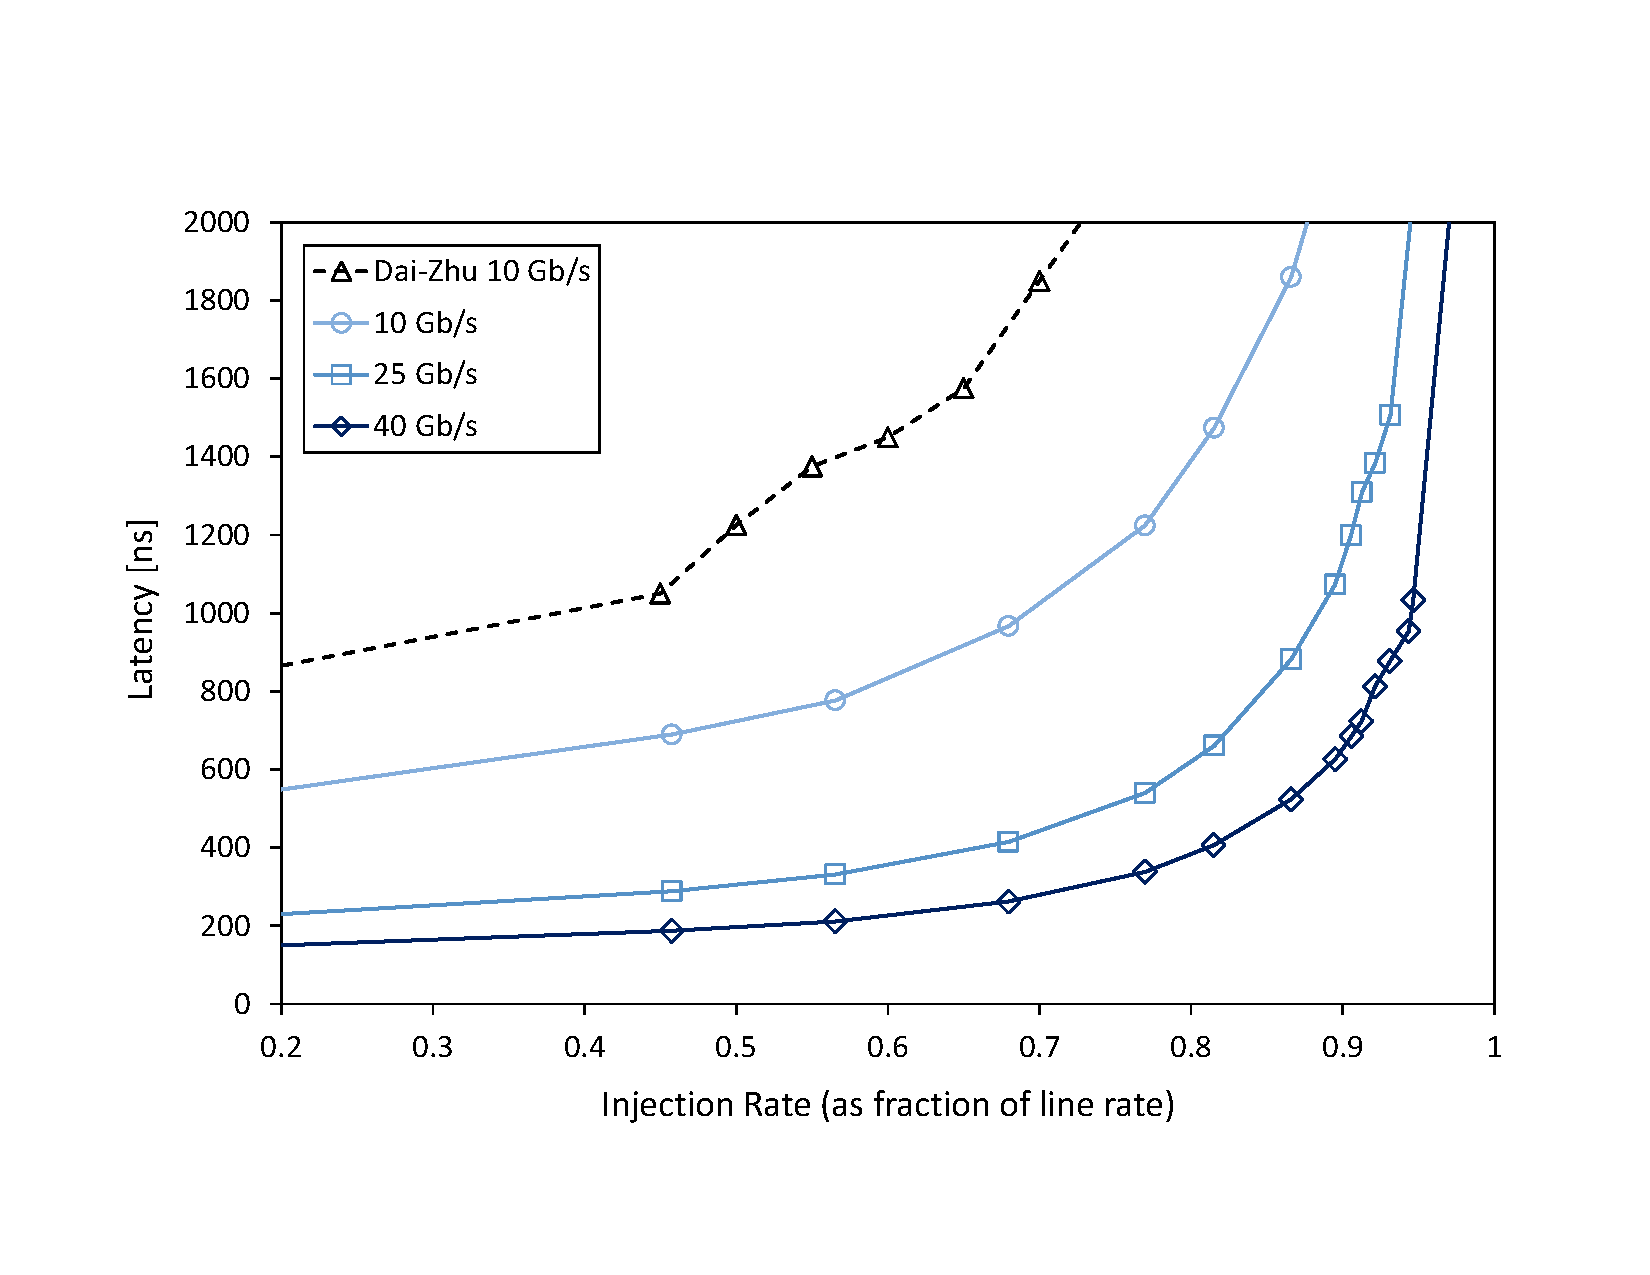
\includegraphics[width=0.485\textwidth, trim = 2cm 2.5cm 2cm 3.4cm, clip]{images/latency-chart-data-320-640.pdf}
\caption{Latency vs. injection rate of the NoC-based Ethernet switch design given line rates of 10, 25, and 40~Gb/s, and compared to the Dai/Zhu 16$\times$16 10~Gb/s FPGA switch fabric design~\cite{dai-zhu}. Our switch queues and Dai/Zhu's switch queues are of size 60kb and 16kb, respectively.}
\label{fig:lat-plot}
\vspace{0cm}
\end{figure}

The average latency of our Ethernet switch design is measured using the \texttt{RTL2Booksim} simulator.
An ON/OFF injection process is used to model bursty, uniform random traffic, with a fixed Ethernet frame size of 512 bytes (as was used in~\cite{dai-zhu}).
Latency is measured as the time between a packet head being injected into the input queue and it arriving out of the output queue.
%The design is simulated at 10, 25, and 40~Gb/s to model modern Ethernet bandwidths, with latency measured and plotted in Fig.~\ref{fig:lat-plot}.
Fig.~\ref{fig:lat-plot} plots the latency of our Ethernet switch at its supported line rates of 10~Gb/s, 25~Gb/s and 40~Gb/s.
Surprisingly, the latency of a 512~byte packet improves at higher line rates.
This is because a higher line rate means a faster rate of injecting NoC flits, and the NoC can handle the extra switching without a large latency penalty thus resulting in an improved overall latency.
%Because the latency of the NoC varies little when the injection bandwidth is below its capacity, NoC-based Ethernet switches of higher throughput inject packets into the NoC at a faster rate and therefore achieve better latency.
No matter what the injection bandwidth, the NoC-based switch considerably outperforms the Dai/Zhu switch~\cite{dai-zhu} for all injection rates.
%The saturation point can be improved by increasing the size of the output queues.
%However, higher throughputs cause the NoC to reach its saturation point at a lower injection rate than lower throughputs.
By supporting these high line rates, our results show that an embedded NoC can push FPGAs into new communication network markets that are currently dominated by ASICs.

%want to say something about programmability being important in these markets, hence the cavium switch.

%Fig.~\ref{fig:lat-plot} plots the latency for both queue depths as a function of the injection rate.
%The ``knee'' in each plot indicates the injection rate at which the output queues become full and start backpressuring the NoC.
%An output queue fills up when it is being driven by multiple sources at the same time, as it can only eject flits at up to the line rate.
%Up until the plot knee, the average latency remains below 65 RTL cycles (156.25 MHz), or 416 ns.

%
%\subsection{On-Chip Memory \textit{(Latency-insensitive, memory-mapped)}}
%\input{memapp}
%
%
%#############################################################
\section{Conclusion}
%-0-0-0-0-0-0-0-0-0-0-0-0-0-0-0-0-0-0-0-0-0-0-0-0-0-0-0-0-0-0-
%
%
%

We proposed augmenting FPGAs with an embedded NoC and focused on how to use the NoC for transporting data in FPGA applications of different design styles.
The FabricPort is a flexible interface between the embedded NoC and the FPGA's core; it can bridge any fabric frequency and data width up to 600~bits to the faster but narrower NoC at 1.2~GHz and 150~bits.
We have shown that latency-insensitive systems can be interconnected using an embedded NoC with lower hardware overhead by taking advantage of the NoC's built-in buffering.
Additionally, we showed how latency-sensitive systems can be guaranteed fixed delay and throughput through the NoC by using Permapaths.

We investigated two streaming applications; latency-sensitive JPEG that only requires wires between modules, and a latency-insensitive Ethernet switch that requires heavy arbitration and switching between its transceiver modules.
With an embedded NoC, JPEG's frequency can be improved by 10--80\%\comment{ compared to the FPGA's traditional interconnect with and without pipelining}.
Wire utilization is also improved, as the embedded NoC avoids wiring hotspots and reduces the use of scarce long wires by 40\% at the expense of a 10\% increase of the much more plentiful short wires.
Finally, we showed that high-bandwidth Ethernet switches can be efficiently constructed on the FPGA; by leveraging an embedded NoC we created an 819~Gb/s programmable Ethernet switch -- a major improvement over the 160~Gb/s achieved by prior work in a traditional FPGA.

%
%

%
%
%\comment{
%#############################################################
\section{Acknowledgments}
%-0-0-0-0-0-0-0-0-0-0-0-0-0-0-0-0-0-0-0-0-0-0-0-0-0-0-0-0-0-0-
%
We are indebted to Prof. Natalie Enright-Jerger and her research team (Shehab Elsayed, Mario Badr and Robert Hesse) for NoC discussions and for providing some of the code used to build \texttt{RTL2Booksim}.
We would also like to thank David Lewis, Mike Hutton, Dana How and Desh Singh for feedback on FPGAs, and Kevin Murray for feedback on latency-insensitive design.
This work is funded by Altera, NSERC and Vanier CGS.

\newpage
%}
%
%
% The following two commands are all you need in the
% initial runs of your .tex file to
% produce the bibliography for the citations in your paper.
\begin{small}

\bibliographystyle{abbrv}

\bibliography{fpga15} 

\end{small}

\end{document}

